\chapter{Competencias}

\section{Análisis FODA}

\subsection{Fortalezas (Factores internos positivos)}

\subsubsection*{F1. Automatización del análisis de infraestructura}

La solución automatiza el proceso de recopilación de información, análisis de métricas y detección de anomalías, reduciendo el esfuerzo manual requerido por los administradores de infraestructura.

\subsubsection*{F2. Uso de Machine Learning}

La utilización del algoritmo Isolation Forest permite detectar comportamientos anómalos sin necesidad de disponer de datos previamente etiquetados, facilitando su aplicación en entornos cloud donde este tipo de información suele ser limitada.

\subsubsection*{F3. Integración con Infraestructura como Código}

La generación automática de una representación de la infraestructura en Terraform permite que las recomendaciones puedan traducirse en cambios concretos sobre la configuración de la infraestructura.

Esta es una fortaleza muy importante porque actualmente la mayoría de herramientas comerciales solo muestran recomendaciones.

\subsubsection*{F4. Validación por parte del usuario}

La solución mantiene al administrador como responsable de aprobar o rechazar cada recomendación antes de modificar la infraestructura.

Esto disminuye el riesgo operativo.

\subsubsection*{F5. Arquitectura modular}

La separación entre:
\begin{itemize}
\item conexión cloud
\item obtención de métricas
\item análisis mediante IA
\item generación de recomendaciones
\end{itemize}

facilita la incorporación de nuevos proveedores cloud o nuevos algoritmos de detección.

\subsection{Oportunidades (Factores externos positivos)}

\subsubsection*{O1. Crecimiento del mercado Cloud}

Cada vez más organizaciones migran sus aplicaciones hacia plataformas cloud, aumentando la necesidad de herramientas de monitoreo y optimización.

\subsubsection*{O2. Adopción de Infraestructura como Código}

Terraform se ha convertido en uno de los estándares más utilizados para administrar infraestructura cloud, favoreciendo soluciones que puedan integrarse con este tipo de tecnologías.

\subsubsection*{O3. Crecimiento de AIOps}

Existe un interés creciente por incorporar técnicas de Inteligencia Artificial para automatizar tareas de operación y monitoreo de infraestructuras.

\subsubsection*{O4. Optimización de costos cloud}

Muchas organizaciones buscan reducir gastos asociados al sobredimensionamiento de recursos, creando una oportunidad para herramientas que identifiquen configuraciones ineficientes.

\subsubsection*{O5. Evolución de las APIs Cloud}

Los proveedores cloud ofrecen cada vez más servicios y métricas accesibles mediante APIs, facilitando el desarrollo de soluciones de análisis automatizado.

\subsection{Debilidades (Factores internos negativos)}

\subsubsection*{D1. Dependencia inicial de Huawei Cloud}

La solución fue diseñada para trabajar con Huawei Cloud, limitando su utilización en organizaciones que emplean otros proveedores.

\subsubsection*{D2. Dependencia de la calidad de los datos}

La precisión del modelo depende directamente de la calidad y disponibilidad de las métricas obtenidas desde la infraestructura.

\subsubsection*{D3. Limitaciones del algoritmo}

Isolation Forest permite detectar comportamientos anómalos, pero no identifica automáticamente la causa que originó la anomalía.

\subsubsection*{D4. Cobertura limitada de recomendaciones}

Las recomendaciones estarán basadas en un conjunto de reglas previamente definidas, por lo que podrían existir situaciones que requieran intervención manual.

\subsubsection*{D5. Necesidad de entrenamiento previo}

El modelo requiere un proceso previo de entrenamiento utilizando datos de un dataset.

\subsection{Amenazas (Factores externos negativos)}

\subsubsection*{A1. Evolución de herramientas comerciales}

Los principales proveedores cloud incorporan continuamente nuevas funcionalidades de monitoreo y optimización que podrían reducir la diferenciación de la solución.

\subsubsection*{A2. Cambios en las APIs}

Las modificaciones en las APIs de Huawei Cloud podrían requerir actualizaciones frecuentes del sistema.

\subsubsection*{A3. Aparición de nuevos algoritmos}

La evolución de nuevas técnicas de detección de anomalías podría ofrecer mejores resultados que Isolation Forest.

\subsubsection*{A4. Restricciones de acceso a métricas}

Algunas organizaciones limitan el acceso a información de monitoreo por cuestiones de seguridad, reduciendo la capacidad de análisis de la solución.

\subsubsection*{A5. Dependencia tecnológica}

La solución depende del correcto funcionamiento de servicios externos como Huawei Cloud y Terraform.

\section{Las 4 P del marketing}

\subsection{Producto}

El producto propuesto consiste en una plataforma web orientada a la optimización de infraestructuras cloud, diseñada para asistir a administradores de infraestructura, equipos DevOps y organizaciones que buscan mejorar el aprovechamiento de sus recursos computacionales. La solución integra técnicas de aprendizaje automático con un motor de recomendaciones para identificar recursos potencialmente mal dimensionados y proponer alternativas de optimización que contribuyan a mejorar el rendimiento de la infraestructura y reducir los costos asociados a su operación.

Uno de los principales diferenciales del producto radica en la combinación de la detección de anomalías mediante técnicas de aprendizaje automático con la utilización de Infraestructura como Código (Infrastructure as Code - IaC). A partir de la información recuperada desde el proveedor cloud, la plataforma construye una representación equivalente de la infraestructura utilizando Terraform, sobre la cual se aplican las recomendaciones generadas por el sistema. Este enfoque permite que las propuestas de optimización no se limiten a una descripción textual, sino que puedan materializarse en una nueva versión de la infraestructura como código, facilitando su revisión, versionado e implementación dentro de los procesos DevOps de la organización.

Desde la perspectiva del cliente, el producto ofrece una herramienta de apoyo a la toma de decisiones que automatiza actividades que tradicionalmente requieren un análisis manual de métricas y un elevado conocimiento técnico. La detección temprana de recursos sobredimensionados o subdimensionados permite optimizar el consumo de infraestructura, mientras que el proceso de validación de recomendaciones mantiene al administrador como responsable final de aprobar los cambios antes de su aplicación. De esta forma, la plataforma busca complementar la experiencia del personal técnico, proporcionando información objetiva que facilite la planificación y ejecución de mejoras sobre la infraestructura cloud.

Finalmente, el producto ha sido concebido bajo una arquitectura modular que favorece su evolución y escalabilidad. Si bien la implementación inicial se orienta al ecosistema de Huawei Cloud, la separación entre los componentes encargados de la obtención de información, el análisis mediante aprendizaje automático, el motor de recomendaciones y la generación de Terraform permite incorporar nuevos proveedores cloud o sustituir los algoritmos de análisis con un impacto mínimo sobre el resto de la solución. Esta característica no solo incrementa la vida útil del producto, sino que también fortalece su potencial de adopción en un mercado caracterizado por la diversidad de plataformas y la constante evolución tecnológica.

\subsection{Precio}

La estrategia de precios propuesta toma como referencia el modelo de comercialización utilizado por herramientas líderes del mercado como Datadog, Dynatrace y New Relic, las cuales ofrecen sus servicios bajo un esquema de \textbf{Software como Servicio (SaaS)} mediante suscripciones periódicas. En estos casos, el costo del servicio se determina principalmente en función de la cantidad de recursos monitoreados, el volumen de datos procesados o las funcionalidades contratadas. Sin embargo, estas plataformas requieren, en la mayoría de los casos, la instalación de agentes sobre los sistemas o la infraestructura del cliente para recopilar métricas en tiempo real, lo que incrementa la complejidad de implementación y las orienta principalmente a organizaciones con necesidades avanzadas de observabilidad.

La solución propuesta adopta un modelo de suscripción similar, pero con una menor barrera de entrada. A diferencia de las herramientas mencionadas, la plataforma obtiene la información necesaria mediante las APIs del proveedor cloud, sin requerir la instalación de agentes adicionales sobre la infraestructura. Esto simplifica significativamente el proceso de adopción, reduce el esfuerzo inicial de implementación y permite que pequeñas y medianas empresas puedan acceder a funcionalidades de análisis y optimización sin incorporar componentes adicionales a sus entornos productivos.

Como estrategia de comercialización, la plataforma adoptará un modelo \textbf{Freemium}, permitiendo que los potenciales clientes evalúen el funcionamiento de la solución antes de contratar un plan de pago. El \textbf{Plan Freemium} ofrecerá la posibilidad de conectar una cuenta cloud y analizar hasta tres recursos por 60 días, generando recomendaciones básicas y permitiendo al usuario familiarizarse con las principales funcionalidades de la plataforma. Esta modalidad busca reducir la barrera de entrada y facilitar la adopción inicial del producto sin necesidad de realizar una inversión económica.

A partir de esta capa gratuita, la plataforma ofrecerá tres niveles de suscripción adaptados a las necesidades de distintos tipos de organizaciones. El \textbf{Plan Starter (10 dólares)} estará orientado a pequeñas y medianas empresas que administren hasta diez recursos cloud, incorporando análisis ilimitados, almacenamiento del historial de recomendaciones y generación de versiones optimizadas de Terraform. El \textbf{Plan Professional (50 dólares)} estará destinado a organizaciones con infraestructuras de mayor tamaño, permitiendo administrar hasta veinticinco recursos e incorporando funcionalidades adicionales como exportación de informes, programación automática de análisis y estadísticas históricas de utilización. Finalmente, el \textbf{Plan Enterprise (a definir)} estará dirigido a grandes organizaciones, ofreciendo la administración de recursos ilimitados, gestión de múltiples proyectos y organizaciones, acceso mediante API para integraciones con otras herramientas, soporte técnico prioritario y funcionalidades avanzadas de auditoría.

Este esquema de comercialización permite que el costo del servicio evolucione de forma proporcional al tamaño de la infraestructura administrada y al valor generado para cada cliente. A medida que aumenta la cantidad de recursos gestionados, también crece el potencial de ahorro derivado de la optimización de la infraestructura, justificando la incorporación de funcionalidades avanzadas y planes de mayor capacidad. De esta manera, la estrategia de precios acompaña el crecimiento de las organizaciones, permitiendo que la plataforma evolucione junto con las necesidades de sus clientes y mantenga un modelo de ingresos recurrentes alineado con las prácticas comerciales predominantes en la industria del software como servicio.

La estrategia de precios propuesta no solo busca establecer un modelo de ingresos recurrentes, sino también reforzar el posicionamiento de la plataforma como una solución de optimización de infraestructura cloud de rápida adopción y bajo impacto operativo. A diferencia de otras herramientas del mercado que requieren la instalación de agentes para realizar un monitoreo continuo, la solución desarrollada obtiene la información necesaria directamente desde los servicios del proveedor cloud, permitiendo analizar la infraestructura y generar recomendaciones de optimización sin introducir componentes adicionales en los entornos del cliente. Esta característica constituye un diferencial competitivo, especialmente para organizaciones que administran infraestructuras privadas o con políticas estrictas de seguridad, donde la incorporación de agentes de terceros puede representar una limitación técnica u operativa.

\subsection{Plaza}

La estrategia de distribución de la solución se basa en un modelo Software como Servicio (SaaS), mediante el cual la plataforma se encuentra disponible a través de una aplicación web accesible desde cualquier ubicación con conexión a Internet. Este enfoque elimina la necesidad de realizar instalaciones locales o desplegar infraestructura adicional por parte del cliente, permitiendo que el proceso de adopción se limite a la creación de una cuenta y la vinculación de su proveedor cloud. Como resultado, se reducen tanto los tiempos de implementación como los costos asociados a la puesta en marcha de la solución.

Además del modelo SaaS propuesto para pequeñas y medianas organizaciones, la plataforma podría ofrecer una modalidad de implementación On-Premise destinada a empresas con políticas estrictas de seguridad o confidencialidad de la información. En este esquema, tanto la aplicación como la base de datos se instalan dentro de la infraestructura del cliente, garantizando que el historial de análisis, las recomendaciones generadas y la información de la infraestructura permanezcan bajo su control y no sean almacenados en servicios administrados por terceros. Esta modalidad amplía el mercado objetivo y permite atender organizaciones pertenecientes a sectores altamente regulados, como el financiero, el gubernamental o el sanitario.

El mercado objetivo está conformado por organizaciones que administran infraestructuras cloud y buscan optimizar el uso de sus recursos computacionales. En una primera etapa, la plataforma se orienta a empresas que utilizan Huawei Cloud, aprovechando la integración desarrollada con los servicios y APIs del proveedor. No obstante, la arquitectura modular de la solución permite incorporar en el futuro soporte para otros proveedores de servicios cloud, como AWS, Microsoft Azure o Google Cloud Platform, ampliando el alcance comercial y permitiendo acceder a un mercado significativamente mayor.

Desde el punto de vista comercial, la plataforma podría distribuirse directamente a través de su sitio web oficial, donde los clientes tendrían la posibilidad de registrarse, acceder al plan Freemium y contratar los distintos niveles de suscripción disponibles. Este canal de venta directa reduce la dependencia de intermediarios, facilita la actualización continua del producto y permite establecer una relación permanente con los clientes mediante la prestación del servicio y el soporte técnico.

Como estrategia de expansión, la solución también podría incorporarse a marketplaces especializados en servicios cloud, como Huawei Cloud Marketplace, AWS Marketplace o Azure Marketplace, una vez que disponga de compatibilidad con dichos proveedores. Estos canales representan una oportunidad para aumentar la visibilidad del producto y facilitar su adopción por organizaciones que ya utilizan estos ecosistemas tecnológicos, aprovechando la confianza y el alcance comercial que ofrecen estas plataformas.

Adicionalmente, la comercialización podría complementarse mediante alianzas estratégicas con consultoras especializadas en transformación digital, proveedores de servicios administrados (Managed Service Providers) y empresas dedicadas a la implementación de soluciones DevOps. Estas organizaciones podrían incorporar la plataforma como parte de su cartera de servicios, ofreciendo a sus clientes una herramienta de apoyo para el análisis y la optimización continua de sus infraestructuras cloud. De esta manera, la estrategia de distribución combina canales digitales directos con alianzas comerciales que permiten ampliar el alcance del producto y favorecer su posicionamiento dentro del mercado de soluciones para la gestión de infraestructura cloud.

\subsection{Promoción}

La estrategia de promoción de la solución se orienta al mercado \textbf{Business to Business (B2B)}, ya que el producto está dirigido a organizaciones que administran infraestructuras cloud, equipos DevOps, administradores de infraestructura y consultoras especializadas en servicios tecnológicos. A diferencia de los productos de consumo masivo, la decisión de adoptar una herramienta de este tipo se fundamenta principalmente en criterios técnicos y económicos, por lo que las acciones de promoción deben enfocarse en demostrar el valor que la plataforma aporta en términos de optimización de recursos, reducción de costos y simplificación de las tareas de administración.

Uno de los principales ejes de la estrategia de promoción consiste en destacar los elementos diferenciadores de la solución frente a las alternativas disponibles en el mercado. En particular, la plataforma combina técnicas de aprendizaje automático para identificar recursos potencialmente mal dimensionados con la generación de recomendaciones sobre una representación de la infraestructura mediante Terraform, sin requerir la instalación de agentes propios sobre los recursos del cliente. Este enfoque permite reducir la complejidad de adopción y ofrecer una propuesta de valor claramente diferenciada respecto de herramientas de observabilidad tradicionales, cuyo objetivo principal es el monitoreo continuo de la infraestructura.

Como mecanismo para incentivar la adopción inicial, el modelo Freemium constituye una herramienta de promoción en sí misma, permitiendo que potenciales clientes utilicen la plataforma con una cantidad limitada de recursos antes de contratar un plan de pago. Esta estrategia disminuye la incertidumbre asociada a la incorporación de una nueva solución tecnológica, ya que las organizaciones pueden evaluar la calidad de las recomendaciones generadas y comprobar los beneficios obtenidos sobre su propia infraestructura antes de realizar una inversión económica.

La difusión del producto debería apoyarse principalmente en canales especializados donde se concentra el público objetivo. Entre ellos se destacan redes profesionales como LinkedIn, comunidades DevOps y Cloud Computing, eventos tecnológicos, conferencias sobre infraestructura cloud y automatización, así como la publicación de artículos técnicos y casos de estudio que demuestren el funcionamiento de la plataforma. Estas acciones permiten aumentar la visibilidad del producto entre profesionales y responsables de la toma de decisiones dentro de las organizaciones, fortaleciendo su posicionamiento como una herramienta especializada en la optimización de infraestructuras cloud.

Finalmente, una estrategia de promoción efectiva debe centrarse en comunicar los beneficios económicos que la solución puede generar para las organizaciones. La posibilidad de identificar recursos sobredimensionados, optimizar su utilización y reducir costos operativos constituye un argumento de alto valor para empresas que buscan maximizar el retorno de sus inversiones en infraestructura cloud. Complementariamente, la generación automática de una versión optimizada de la infraestructura mediante Terraform y la eliminación de la necesidad de instalar agentes propios representan ventajas competitivas que contribuyen a diferenciar la plataforma dentro de un mercado caracterizado por la creciente demanda de soluciones inteligentes para la gestión de infraestructura.

\section{Análisis de las Cinco Fuerzas de Porter}

\subsection{Rivalidad entre competidores existentes}

El mercado de herramientas para la administración y optimización de infraestructuras cloud presenta un alto nivel de competencia debido a la presencia de proveedores consolidados como Datadog, Dynatrace, New Relic y las soluciones nativas ofrecidas por AWS, Microsoft Azure, Google Cloud y Huawei Cloud. Estas plataformas cuentan con una amplia trayectoria, una importante base de clientes y una gran inversión en investigación y desarrollo, lo que representa una barrera significativa para nuevos participantes.

No obstante, la competencia se concentra principalmente en herramientas de observabilidad y monitoreo continuo, cuyo funcionamiento suele depender de la instalación de agentes para la recopilación de métricas y está orientado a ofrecer una visión integral del estado de la infraestructura. En este contexto, la solución propuesta busca diferenciarse mediante un enfoque especializado en el análisis del dimensionamiento de recursos y la generación de recomendaciones sobre Infraestructura como Código (IaC), reduciendo la complejidad de implementación al obtener la información directamente desde las APIs del proveedor cloud.

En consecuencia, si bien la rivalidad competitiva es elevada, existe una oportunidad para posicionar la solución dentro de un segmento específico del mercado, orientado a organizaciones que buscan optimizar sus recursos cloud mediante una herramienta de rápida adopción y con una menor dependencia de componentes adicionales.

\subsection{Amenaza de nuevos competidores}

El desarrollo de soluciones destinadas a la optimización de infraestructuras cloud requiere conocimientos especializados en tecnologías cloud, aprendizaje automático, monitoreo de infraestructura, automatización mediante Infraestructura como Código y arquitecturas distribuidas. Asimismo, resulta necesario disponer de experiencia en la integración con APIs de los distintos proveedores cloud y en el procesamiento de grandes volúmenes de métricas.

Estos requerimientos constituyen barreras técnicas que dificultan el ingreso de nuevos competidores. Sin embargo, el crecimiento sostenido del mercado cloud y la disponibilidad de herramientas y bibliotecas de código abierto reducen parcialmente estas barreras, permitiendo que nuevas empresas desarrollen soluciones innovadoras con una inversión inicial menor que la requerida años atrás.

Por este motivo, la amenaza de nuevos competidores puede considerarse media, siendo fundamental mantener una estrategia de innovación continua que permita incorporar nuevos algoritmos, funcionalidades y proveedores cloud para conservar una ventaja competitiva.

\subsection{Poder de negociación de los clientes}

Los potenciales clientes cuentan con un elevado poder de negociación (alto) debido a la amplia oferta de herramientas disponibles para el monitoreo y la administración de infraestructuras cloud. La existencia de soluciones comerciales consolidadas, así como de herramientas nativas ofrecidas por los propios proveedores cloud, facilita que las organizaciones comparen funcionalidades, costos y modelos de comercialización antes de adoptar una nueva plataforma.

En este escenario, la propuesta de valor de la solución debe centrarse en aquellos aspectos que la diferencian de las alternativas existentes. La posibilidad de detectar recursos potencialmente mal dimensionados mediante técnicas de aprendizaje automático, generar recomendaciones sobre una representación de la infraestructura en Terraform y operar sin requerir la instalación de agentes propios constituyen características que pueden disminuir la sensibilidad del cliente frente al precio y favorecer la adopción del producto.

Adicionalmente, la incorporación de un modelo Freemium reduce la barrera de entrada para nuevos usuarios, permitiéndoles evaluar el funcionamiento de la plataforma antes de comprometerse con una suscripción de pago.

\subsection{Poder de negociación de los proveedores}

El funcionamiento de la solución depende principalmente de los servicios y APIs ofrecidos por el proveedor cloud, ya que estos constituyen la fuente de información utilizada para obtener la infraestructura y las métricas necesarias para el análisis. En la implementación propuesta, Huawei Cloud representa el proveedor tecnológico principal, por lo que cambios en sus APIs, políticas comerciales o servicios de monitoreo podrían afectar directamente el funcionamiento de la plataforma.

Asimismo, la solución utiliza Terraform como mecanismo para representar la infraestructura como código, dependiendo de la disponibilidad y evolución de los proveedores oficiales mantenidos por HashiCorp. No obstante, al tratarse de tecnologías ampliamente adoptadas y con documentación pública, el riesgo asociado resulta moderado.

En consecuencia, el poder de negociación de los proveedores puede considerarse bajo, ya que, si bien la solución depende de servicios externos para su funcionamiento, la utilización de estándares ampliamente aceptados y una arquitectura modular permiten reducir el impacto de eventuales cambios tecnológicos.

\subsection{Amenaza de productos sustitutos}

La principal amenaza proviene de las herramientas nativas de optimización desarrolladas por los proveedores cloud, como AWS Compute Optimizer, Azure Advisor o Google Active Assist, las cuales ofrecen recomendaciones específicas para los servicios que administran y cuentan con un alto nivel de integración dentro de sus respectivos ecosistemas.

Sin embargo, estas soluciones suelen encontrarse estrechamente vinculadas a un proveedor específico y, en muchos casos, orientan sus recomendaciones hacia los servicios propios de cada plataforma. La solución propuesta busca diferenciarse mediante un enfoque centrado en el análisis de anomalías para identificar recursos potencialmente mal dimensionados y en la generación de una representación optimizada de la infraestructura mediante Terraform, permitiendo que las recomendaciones puedan integrarse dentro de procesos de Infraestructura como Código.

Además de estas herramientas, también constituyen productos sustitutos las tareas de análisis manual realizadas por administradores de infraestructura y consultoras especializadas. No obstante, estos procesos suelen requerir una mayor inversión de tiempo y dependen significativamente de la experiencia del personal técnico, lo que representa una oportunidad para automatizar parte del proceso de análisis y apoyar la toma de decisiones mediante la plataforma propuesta.

\begin{figure}[htbp]
\centering
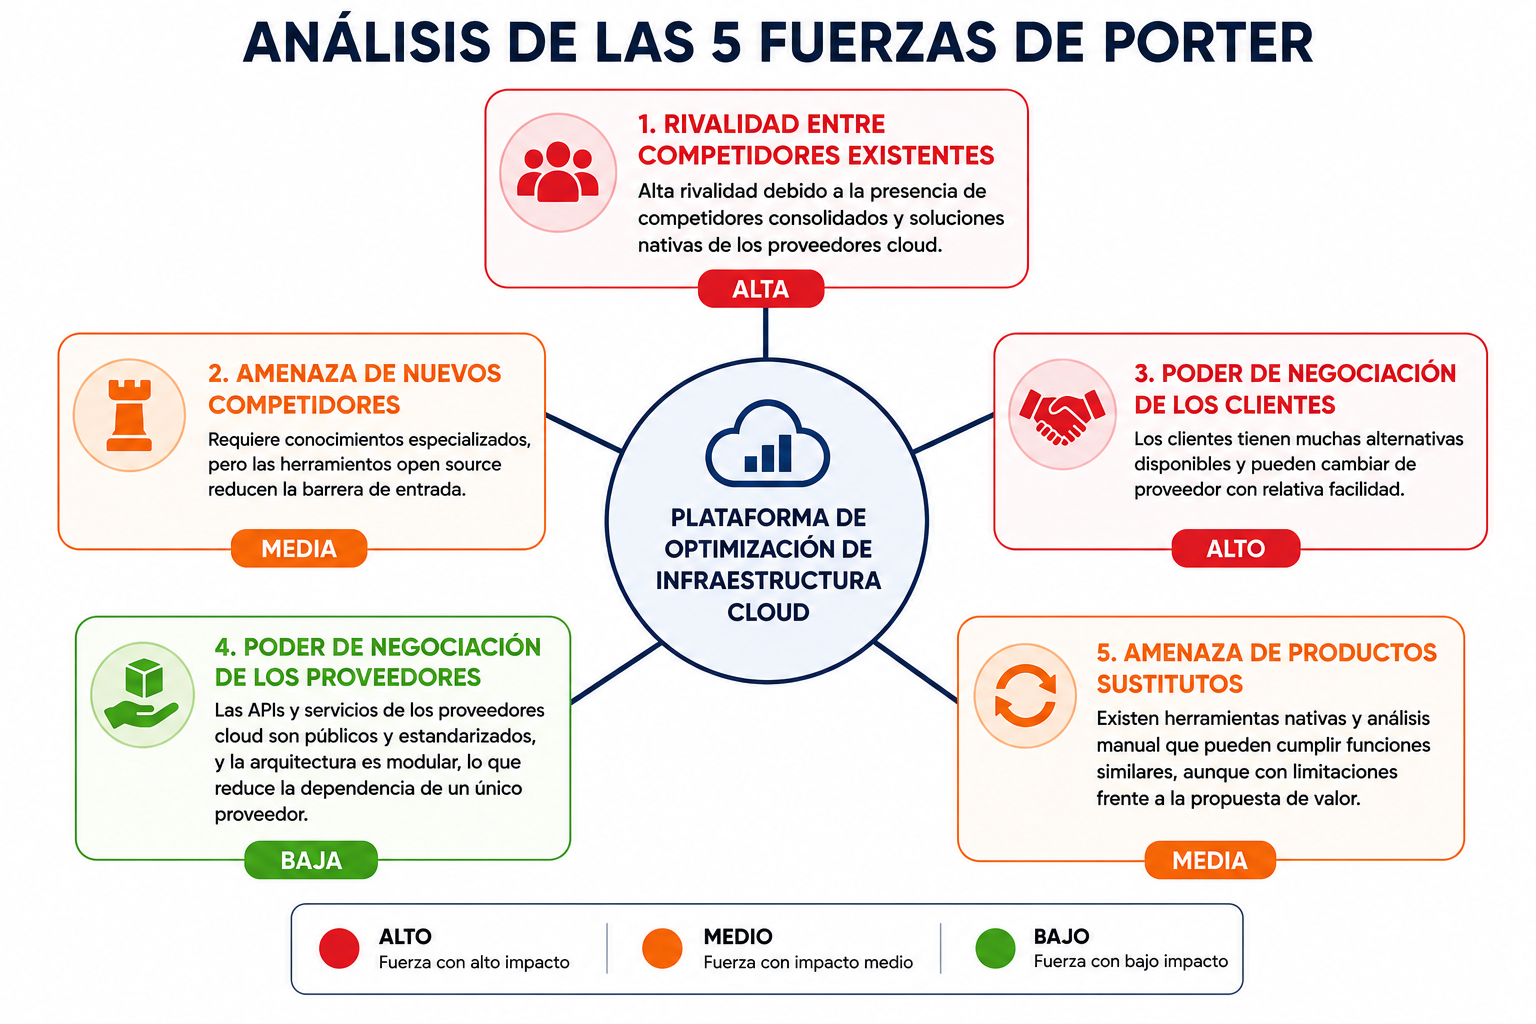
\includegraphics[width=0.9\textwidth]{media/image1.png}
\caption{Análisis de las Cinco Fuerzas de Porter}
\label{fig:porter}
\end{figure}

\section{Estrategia competitiva}

Del análisis realizado mediante las herramientas de marketing estratégico se desprende que el mercado de soluciones para la gestión de infraestructura cloud presenta un elevado nivel de competencia, impulsado principalmente por plataformas consolidadas como Datadog, Dynatrace, New Relic y las herramientas nativas de los principales proveedores cloud. No obstante, dicho análisis también permitió identificar oportunidades para el desarrollo de soluciones especializadas que atiendan necesidades específicas de optimización de infraestructura, diferenciándose de las plataformas orientadas principalmente a la observabilidad y el monitoreo continuo.

En este contexto, la estrategia competitiva de la solución se basa en la \textbf{diferenciación}. En lugar de competir directamente con herramientas de observabilidad de propósito general, la plataforma se posiciona como una solución especializada en la detección de recursos potencialmente mal dimensionados y en la generación de recomendaciones de optimización sobre Infraestructura como Código (IaC). Esta propuesta de valor combina técnicas de aprendizaje automático para identificar comportamientos anómalos con la generación automática de configuraciones en Terraform, facilitando la incorporación de las recomendaciones dentro de los procesos de administración y automatización de infraestructura.

Desde el punto de vista tecnológico, uno de los principales factores diferenciadores consiste en la obtención de información directamente desde las APIs del proveedor cloud, evitando la necesidad de instalar agentes propios sobre la infraestructura del cliente. Esta característica reduce la complejidad de implementación, disminuye el impacto operativo y favorece la adopción de la solución en organizaciones que administran entornos con políticas estrictas de seguridad o que buscan minimizar la incorporación de componentes adicionales en sus arquitecturas.

La estrategia comercial acompaña este posicionamiento mediante un modelo de distribución SaaS y un esquema Freemium, permitiendo que potenciales clientes evalúen el funcionamiento de la plataforma sin realizar una inversión inicial. Este enfoque reduce las barreras de adopción y facilita la incorporación progresiva de organizaciones de distintos tamaños, mientras que los planes de suscripción escalonados permiten que el crecimiento de los ingresos acompañe la expansión de la infraestructura administrada por cada cliente.

La estrategia propuesta no busca competir por amplitud de funcionalidades frente a las grandes plataformas de observabilidad, sino por la especialización en un problema concreto: la optimización inteligente del dimensionamiento de recursos cloud. La combinación de aprendizaje automático, generación de recomendaciones sobre Infraestructura como Código, ausencia de agentes propios y un modelo comercial de baja barrera de entrada constituye una propuesta de valor diferenciada que permite posicionar a la solución como una alternativa innovadora dentro del mercado de herramientas para la administración y optimización de infraestructuras cloud.
